\apendice{Especificación de diseño}
\section{Introducción}
En este punto se detalla cómo se han resuelto las especificaciones expresadas anteriormente.
\section{Diseño de datos}

Cabe recordar que este proyecto tiene la particularidad de que los elementos domóticos y lumínicos vuelven al estado de reposo al terminar el día y la programación diaria se realiza desde la posición de reposo.

El proyecto se divide en dos grupos funcionales: 
El primer grupo funcional se encarga de la obtención de datos del exterior y tratar estas cadenas de texto como json, y el otro grupo se basa en el tratamiento de cadenas de texto enviadas por el usuario mediante el bot de Telegram que hemos creado para la ocasión.

Ambas partes tienen un punto en común; éste es el archivo de configuración que contiene las credenciales y es dónde se plasma la arquitectura física entre los diferentes periféricos. El archivo se encuentra un nivel por encima del repositorio compartido en la carpeta <<credentials>> con el nombre <<config2.bot>>.~\\

La estructura del archivo será la expuesta en el Listing~\ref{Config2.bot}:~\\~\\
\begin{lstlisting}[language=Python, caption={Estructura del archivo de configuración general de la \mbox{arquitectura}.\\}, basicstyle=\small, label={Config2.bot}]
# Introduce tu Token aqui:
AQUI: TOKENBOT

# Introduce los usuarios autorizados separados por comas:
AQUI: USUARIO1, USUARIO2, ETC

# Key Climacell
AQUI: CLIMACELLKEY

# Key KeyWeatherapi
AQUI: WEATHERAPIKEY

#--------------------------------------------------------
# Numero de persianas [Situacion, PinSubir, PinBajar]
AQUI: EL NUMERO DE PERSIANAS A CONTROLAR
AQUI: SITUACION PINSUBIR PINBAJAR

#--------------------------------------------------------
# Numero de luces  [Situacion, Pin]
AQUI: EL NUMERO DE LUCES A CONTROLAR
AQUI: NOMBRE PINCONTROL

#--------------------------------------------------------
# Pin caldera [Situacion, Pin]
1
AQUI: NOMBRE PINCONTROL
\end{lstlisting}


Por un lado, el grupo funcional automático, llama a las APIS externas y guarda los datos en dos archivos antes de ser procesados y volcados al Cron. Para obtener los tokens, se sirve de la función \texttt{obtencionDatos.py} que lee la información del archivo anterior y calcula las rutas necesarias para el correcto funcionamiento del Sistema.

En este punto, de forma general, se recaba la información de forma automática llamando a las APIS aunque también se puede recopilar la información bajo petición del usuario.

El primer archivo, se llama <<InfoRecabada>> y es el archivo donde se almacenan los datos de las consultas en formato json. Posteriormente, se genera el archivo <<log.cron>>, que nos presenta los datos junto a otros para que podamos obtenerlos cuando queramos desde el bot. Ambos archivos necesitan ser leídos y tratados como <<string>>.

Por otro lado, tenemos la parte del Sistema que nos permite operar contra éste con órdenes de carácter inmediato desde el FrontEnd de Telegram, pasando por su API hasta el <<listener>>; que es la parte de nuestro bot (que está corriendo continuamente) que está diseñado para leer el texto que le enviamos y actuar según tengamos programado en el archivo de configuración del bot. Esta configuración podemos verla en la imagen~\ref{SecuenciaAcciones}. 

\begin{figure}[h]
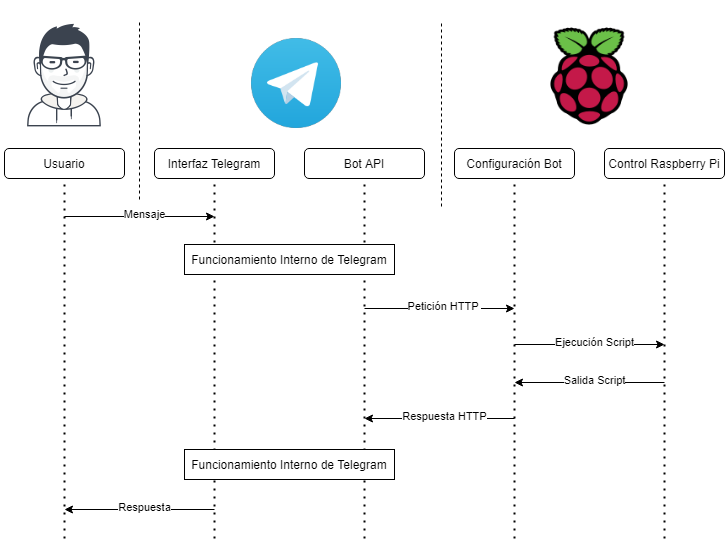
\includegraphics[width=1.15\textwidth]{img/Diagramas/FuncionamientoBot.png}
\caption{Secuencia de acciones.}\label{SecuenciaAcciones}
\end{figure}

\section{Diseño procedimental}
En este punto se recogen los detalles más importantes en la ejecución las órdenes de nuestro Sistema, tanto la parte automática como la parte bajo demanda. Existen tres tipos de posibles llamadas de interacción desde el usuario, éstas son: órdenes a la máquina, órdenes a los periféricos y órdenes para recopilar datos de las APIS. Estos tres tipos de llamadas se han ilustrado en la figura~\ref{SecAcSys}. También podemos ver el flujo de comunicación entre las diferentes partes del software en la imagen~\ref{Arquitectura}.

\begin{figure}[h]
\centering
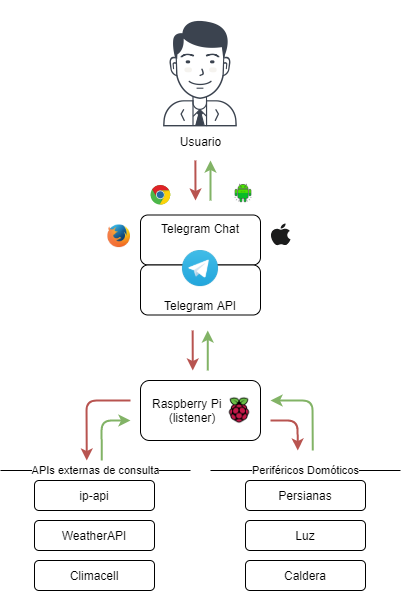
\includegraphics[width=0.8\textwidth]{img/Diagramas/arquitectura.png}
\caption{Diagrama de comunicación.}\label{Arquitectura}
\end{figure}


\begin{landscape}
\imagenAncho{img/Diagramas/DiagSecSys.png}{Diagrama de secuencia de acciones del sistema.}{1.25}\label{SecAcSys}
\end{landscape}

\section{Diseño arquitectónico}

El diseño arquitectónico de nuestro sistema se basa en la intergación de diferentes microservicios independientes entre sí a nivel de desarrollo. Esto se refleja en que nos beneficiamos de unas APIS sin preocuparnos por la lógica del BackEnd permitiéndonos ampliar la carga de trabajo sobre estas APIs. Esto podemos verlo gráficamente en la imagen~\ref{Arquitectura}.

Podemos ver la estructura de los diferentes módulos del software en la imagen~\ref{Paquetes}.

\begin{figure}[h]
\centering
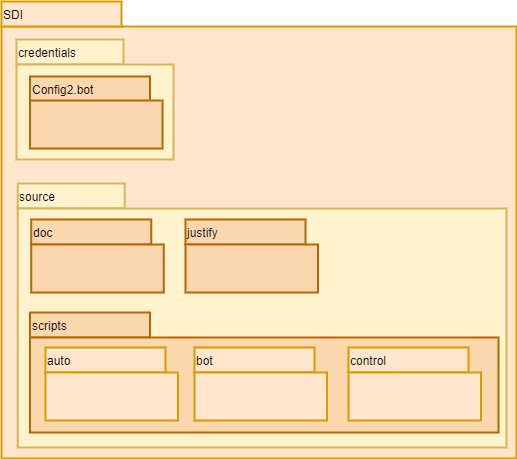
\includegraphics[width=0.8\textwidth]{img/Diagramas/Diagrama de paquetes.png}
\caption{Diagrama de paquetes.}\label{Paquetes}
\end{figure}

Dentro de directorio scripts disponemos de los siguientes archivos de código:
\begin{itemize}
    \item \texttt{obtencionDatos.py}: Lee el archivo de configuración y devuelve los valores de:
    \begin{itemize}
        \item \textbf{tokenBot}: Token del bot de Telegram.
        \item \textbf{users}: Usuarios acreditados.
        \item \textbf{climacellKey}: Token de Climacell.
        \item \textbf{weatherApiKey}: Token de WeatherAPI.
        \item \textbf{persianas}: Información sobre las persianas.
        \item \textbf{luces}: Información sobre las luces.
        \item \textbf{calderas}: Información sobre la caldera.
        \item \textbf{rutaCred}: Ruta al directorio credentials.
        \item \textbf{rutaAuto}: Ruta al directorio auto.
    \end{itemize}
\end{itemize}


En el directorio \texttt{auto} disponemos de los métodos y funciones propios de la parte automática:
\begin{itemize}
    \item \texttt{1\_recabaInfo.py}: Obtiene la información de las APIs externas y la graba en archivos de datos.
    \item \texttt{3\_cocinado.py}: Procesa la información recogida y genera el próximo archivo de configuración de Cron.
    \item \texttt{4\_reescribeCron.py}: Vuelca la nueva configuración y reinicia los servicios de la máquina.
    \item \texttt{LanzaTodoElProceso.sh}: Lanza los tres procesos anteriores.
\end{itemize}

En el directorio \texttt{control} disponemos de los métodos y funciones de control de los periféricos:
\begin{itemize}
    \item \texttt{ApagarCaldera.sh}: Apaga la caldera.
    \item \texttt{EncenderCaldera}: Enciende la caldera.
    \item \texttt{Bajar}: Baja las persianas.
    \item \texttt{Subir}: Sube las persianas.
    \item \texttt{LucesOff}: Apaga las luces.
    \item \texttt{LucesOn}: Enciende las luces.
\end{itemize}

En el directorio \texttt{bot} disponemos de siguientes métodos y funciones que se encargan de realizar las acciones bajo demanda:
\begin{itemize}
    \item \texttt{info(m, bot)}: Llama al método enviándole la orden por Telegram y la información del bot, y nos envía por mensaje información sobre la máquina.
    \item \texttt{generador(m, bot)}: Llama al método enviándole la orden por Telegram y la información del bot, lanza los scripts y nos devuelve la confirmación de la acción.
    \item \texttt{horaSubida(m, bot)}: Llama al método enviándole la orden por Telegram y la información del bot, y nos informa de la hora a la que subirán las persianas y, si el mensaje incluye una hora la modificará. Finalmente nos envía la hora nueva de subida de las persianas.
    \item \texttt{diagrama(m, bot, pwdBot)}: Llama al método enviándole la orden por Telegram, el pwd y la información del bot, para enviar el último diagrama de temperaturas o el que el usuario solicite.
    \item \texttt{datos(m, bot)}: Llama al método enviándole la orden por Telegram y la información del bot, y devuelve las principales horas de interacción del sistema automático.
    \item \texttt{controlPersianas(m, bot)}: Llama al método enviándole la orden por Telegram y la información del bot, y nos permite interactuar con las persianas.
    \item \texttt{calefaccion(m, bot)}: Llama al método enviándole la orden por Telegram y la información del bot, y nos informa de la temperatura a la que se encenderá la caldera, y si se incluye una temperatura se puede modificar. Finalmente envía la temperatura escogida tras grabarla.
    \item \texttt{temperaturas(m, bot)}: Llama al método enviándole la orden por Telegram y la información del bot, y devuelve por mensaje una tabla con las temperaturas por horas, además de la hora a la que suben las persianas y encienden las luces (y posteriormente bajan las persianas).
    \item \texttt{configBot()}: Obtiene los parámetros de configuración gracias a obtencionDatos(), obtiene la hora y la devuelve a todos los usuarios.
        \item \texttt{command\_help(m)}:
    \begin{itemize}
        \item Si \texttt{m} es \textbf{ayuda}, envía el menú de ayuda.
        \item Si \texttt{m} es \textbf{reiniciar}, reinicia la máquina.
        \item Si \texttt{m} es \textbf{apagar}, apaga la máquina.
    \end{itemize}
    \item \texttt{compruebaUsuario(message)}: Comprueba si el remitente del mensaje es un usuario autorizado.
    \item \texttt{command\_default(m)}: Devuelve el mensaje por defecto.
\end{itemize}







































